\subsection{Part Selection}

\noindent For \textbf{obstacle detection}, the final selections are:
\begin{enumerate}
	\item 2x HC-SR04 Multistatic Ultrasonic Sensors for lateral-facing detection.
	\item 2x RCWL-1005 Monostatic Ultrasonic Sensors for front-facing detection.
	\item The TFLuna LiDAR sensor, for its precision and accuracy. Front-facing. It has easy I2C configuration and a great price point, making it a viable option.
	\item The BNO-055 Inertial Measurement Unit because of its advantages like quaternion output and affordability, which greatly enhance FORWARD stability.
\end{enumerate}

% MCU comparison
\begin{table}[H]
	\centering
	\setlength{\tabcolsep}{5pt} % Restore default column padding
	\renewcommand{\arraystretch}{1.75} % Restore default row height
	\scalebox{0.85}{ % Scale down the entire table by 85%
		\begin{NiceTabular}{cccccc}[hvlines,colortbl-like]
			\CodeBefore
			\rowcolor{blizzardblue}{1}
			\Body
			Model            & ESP32D & Raspberry Pi 4 B & Jetson Nano \\
			\hline
			Processor        & Xtensa dual-core     & Broadcom BCM2711 & NVIDIA Maxwell GPU \\
			Memory           & 4MB-8MB Flash/PSRAM  & 1GB-8GB LPDDR4   & 4GB LPDDR4 \\
			Connectivity     & WIFI, Bluetooth      & Wi-Fi, Bluetooth, Ethernet & Ethernet \\
			I/O Ports        & GPIO, UART, I2C, SPI & GPIO, 2 USB 3.0, 2 HDMI & USB 3.0, USB 2.0, HDMI \\
			Power            & 5V (varies)          & 5V DC via USB or GPIO & 5V 4A DC, 5V 2A Micro-USB \\
			Price            & \$5 - \$15           & \$30 - \$50       & \$250 - \$500 \\
		\end{NiceTabular}
	}
	\caption{\label{fig:mcuComparison}Comparison of MCU Options}
\end{table}

\noindent The FORWARD team selects the ESP32 MCU because of it's affordability and I/O ports. This MCU achieves all of our needed functionality at a fraction of the cost of the other products. \\

% Camera comparison
\begin{table}[H]
	\centering
	\setlength{\tabcolsep}{5pt} % Adjust column spacing
	\renewcommand{\arraystretch}{1.75} % Adjust row spacing
	\scalebox{0.8}{ % Scale down the entire table by 85%
		\begin{NiceTabular}{lccc}[hvlines,colortbl-like]
			\CodeBefore
			\rowcolor{blizzardblue}{1} % Row background color for header
			\Body
			Specification             & ESP32 CAM                  & Oak-D Lite                       &  AMB82-Mini\\
			\hline
			Resolution                & 2MP/5MP   & 13 MP (RGB)                      & 1920 x 1080 (Full HD)            \\
			Frame Rate                & 1600x1200/2592x1944       & 4K@30FPS/1080P@60FPS     & 1080P/720P@30FPS           \\
			CPU/MCU                   & ESP32 @ 240 MHz                 & AI Engine, 6-axis sensor         & ARMv8M (500 MHz/0.4 TOPS)   \\
			Memory                    & 520 KB SRAM, 4 MB PSRAM         & N/A                              & 128 MB DDR2                     \\
			Interface                 & Wi-Fi/24-pin Cam Bus        & USB2/USB3                        & WiFi/BT/USB/GPIO    \\
			Price                     & \$10-15                 		& \$199                			& \$25-\$30                     \\
		\end{NiceTabular}
	}
	\caption{\label{fig:compareCameras}Comparison of Camera Modules for ESP32-based Applications}
\end{table}

\noindent The FORWARD team selects the Realtek AMB82-Mini IoT AI Camera because of it's ability to perform all necessary AI processes while still maintaining a cost effective price. It also is a noticeable image quality improvement over the ESP32 Cam. \\

\noindent A stretch requirement of our project is to implement a depth perception capability with our system. Due to the sensor fusion solution that we are taking (using the grid-like field of view described in figure \ref{fig:Grid-Generatio}) we have decided that we no longer need a high quality of camera to obtain the depth data. \\

\begin{table}[H]
	\centering
	\setlength{\tabcolsep}{5pt} % Adjust column spacing
	\renewcommand{\arraystretch}{1.75} % Adjust row spacing
	\scalebox{0.8}{ % Scale down the entire table by 85%
		\begin{NiceTabular}{lccc}[hvlines,colortbl-like]
			\CodeBefore
			\rowcolor{blizzardblue}{1} % Row background color for header
			\Body
			Specification             & Ultralytics YOLO           	& FOMO                    		& Edge Impulse \\
			\hline
			Processing Time           & 6-100 ms                   	& 10-40 ms            			& 10-50 ms \\
			Memory Usage              & Few hundred MB             	& 256 KB                   		& 100 KB-1 MB \\
			Supported Devices         & ESP32, Raspberry Pi, GPU   	& ESP32, Raspberry Pi, GPU		& ESP32, Raspberry Pi, GPU \\
			Training Complexity       & Moderate        			& Moderate                      & High \\
			Cost                      & Free                     	& Free                  	& Free \\


		\end{NiceTabular}
	}
	\caption{\label{fig:aiComparison}Comparison of AI Image Processing Solutions}
\end{table}

\noindent The FORWARD team selects to use the YOLO model family because of it's memory size flexibility from model to model as well as it's user friendly libraries to make integration simple. \\

% Headphones comparison
\begin{table}[H]
	\centering
	\setlength{\tabcolsep}{5pt} % Restore default column padding
	\renewcommand{\arraystretch}{1.75} % Restore default row height
	\scalebox{0.9}{ % Scale down the entire table by 85%
		\begin{NiceTabular}{cccccc}[hvlines,colortbl-like]
			\CodeBefore
			\rowcolor{blizzardblue}{1} % Row background color for header
			\Body
			Model            & Suunto Wing & Shokz OpenRun Pro & YouthWhisper \\
			\hline
			Battery Life     & 6 hours (playtime)     & 10 hours          & 8 hours \\
			Charging Time    & 1.5 hours & 1 hour 	 	& 2 hours \\
			Water Resistance & IPX8                  & IP55              & IPX6 \\
			Connectivity     & Bluetooth 5.0          & Bluetooth 5.1     & Bluetooth 5.0 \\
			Weight           & 45 grams               & 29 grams          & 30 grams \\
			Price            & \$169                 & \$159             & \$35 \\
		\end{NiceTabular}
	}
	\caption{\label{fig:headphonesComparison}Comparison of Headphone Options}
\end{table}

\noindent The FORWARD team selects to use the YouthWhisper Bone Conduction headphones due to their high affordability, solid battery life, and lighter weight. \\

\begin{table}[H]
	\centering
	\setlength{\tabcolsep}{5pt} % Restore default column padding
	\renewcommand{\arraystretch}{2.5} % Restore default row height
	\scalebox{0.55}{ % Scale down the entire table
		\begin{NiceTabular}{|l|c|c|c|c|c|c|c|}[hvlines,colortbl-like]
			\CodeBefore
			\rowcolor{gray!15}{1}
			\Body
			\textbf{Motor} & \textbf{Oumefar8r2gund350 \cite{yzl1}} & \textbf{775 DC Motor \cite{Citphto}} & \textbf{No. 14 \cite{AliExpress1}} & \textbf{SHABEAM A MOTOR \cite{AliExpress2}} & \textbf{P300 \cite{AliExpress3}} & \textbf{MBD65WI \cite{PrecisionMicrodrives}} & \textbf{S55B-150 \cite{AliExpress8}} \\ 
			\hline 
			\textbf{Voltage} & 12V & 24V & 18V & 10.5V-21V & 12V-24V & 21.6V & 21.6V \\ 
			\hline 
			\textbf{Current} & 0.32A & 12A & 8A starting & 3.3A & 7-13A & 10A & 11A (max tested) \\ 
			\hline 
			\textbf{Power} & 150W & 200W & 300W & 300W & 300W & 150W & 150W \\ 
			\hline 
			\textbf{Type} & Brushed & Brushed & Brushless & Brushless & Brushless & Brushless & Brushless \\ 
			\hline 
			\textbf{RPM} & 15000 & 12000 & Unlisted & 31570 & 130000 & Unlisted & Unlisted \\ 
			\hline 
			\textbf{Weight} & 0.77lbs & 0.77lbs & 1.23lbs & Unlisted & 0.52lbs & 0.62lbs & 0.331lbs \\ 
			\hline 
			\textbf{Arrival Time} & 3 days & 2 days & 1-2 weeks & 1-2 weeks & 1-2 weeks & 1-2 weeks & 1-2 weeks \\ 
			\hline 
			\textbf{Price} & \$19.49 & \$12.99 & \$28.03 & \$20.01 & \$42.46 & \$13.83 & \$10.57 \\ 
		\end{NiceTabular}
	}
	\caption{\label{fig:motorSpecifications}Motor Specifications}
\end{table}


\noindent When deciding on what DC motors that we wanted to use, our main concerns were power, current rating, motor type, and price. It was calculated that in order to meet the speed requirements, we needed a total of 300W or 150W per motor. All of the motors investigated thus are at least 150W. It was also preferable to use brushless DC motors, as they are higher in quality (longevity, efficiency, low noise) than brushed DC motors and are more widely compatible with motor drivers. To decide between the brushless DC motors, we mostly looked at price and found the most cost-effective motors, while also keeping in mind the current rating so that we can purchase motor drivers with a large enough current rating to supply the motors. Thus, we decided to use the S55B-150 DC motors. 


\noindent The FORWARD team selects to use \\

\begin{table}[H]
	\centering
	\setlength{\tabcolsep}{5pt} % Restore default column padding
	\renewcommand{\arraystretch}{1.75} % Restore default row height
	\scalebox{0.85}{ % Scale down the entire table by 75%
		\begin{NiceTabular}{|l|c|c|c|}[hvlines,colortbl-like]
			\CodeBefore
			\rowcolor{gray!15}{1}
			\Body
			\textbf{Specification} & \textbf{B0B4SK8M1C \cite{DIANN}} & \textbf{A19090500ux0371 \cite{uxcell}} & \textbf{Vibration Motor \cite{eBayDC}} \\ 
			\hline 
			Voltage & 1.5-3.7V & 4.5-12V & 3-5V \\ 
			\hline 
			Current & 85mA & 250mA & 15mA \\ 
			\hline 
			Type & DC & DC & DC \\ 
			\hline 
			Arrival Time & 4 days & 4 days & 1-3 weeks \\ 
			\hline 
			Price (Qty) & \$5.99 (10) & \$10.99 (2) & \$9.21 (2) \\ 
		\end{NiceTabular}
	}
	\caption{\label{fig:vibrationMotorSpecifications}Vibration Motor Specifications}
\end{table}

\noindent Haptic motors are small DC motors that are used for vibration feedback in the handlebars of the walker. Because they are only used for the purpose of vibration, these motors are very small and do not draw much current. Our main concern with deciding which haptic motors to use is the voltage rating and price. In order to be compatible with most motor drivers, the motors should be able to be operated at both 5V and 3V. Although not the most cost-effective, we chose the "Vibration Motor" as it has the largest compatibility with motor drivers.\\

\begin{table}[H]
	\centering
	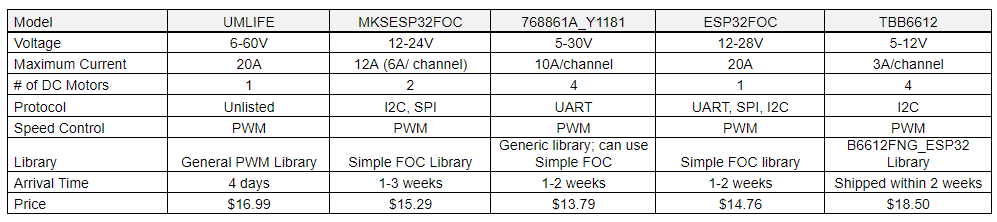
\includegraphics[width=1\textwidth]{./Images/motor_controller_table.png}
	\caption{\label{fig:motor_controller}Motor Controller Specifications}
\end{table}

\noindent After comparing multiple factors, we ultimately chose the 768861A\_Y1181 motor controller. This is because our main concern was supplying current to the motors and operating all 4 motors from the same controller. The motors that we chose to drive the wheels draw up to 11A of current, which the 768861A\_Y1181 would be able to handle, although it is rated for 10A, upon examining the data sheet. This motor controller also provides a wide voltage range of 5-30V, which is able to provide the correct voltage for both the wheel-driving motors and the haptic motors. The 768861A\_Y1181 also happens to be the most cost-effective of the motor controllers. \cite{UMLIFE} \cite{AliExpress5} \cite{Makerbase} \cite{AliExpress7} \cite{CircuitBasics} \cite{Espressif1} \cite{AliExpress4} \cite{Burgess} \cite{RandomNerd} \cite{Espressif2} \cite{SimpleFOC} \cite{SimpleFOC2} \cite{Peza}\\


\begin{table}[H]
	\centering
	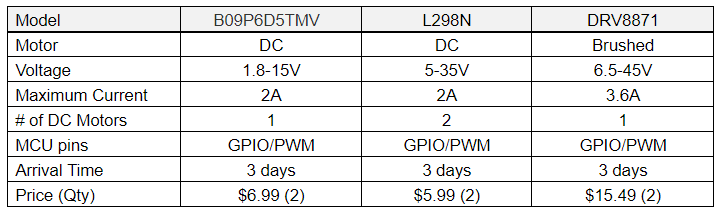
\includegraphics[width=1\textwidth]{./Images/haptic_driver_table_2.png}
	\caption{\label{fig:haptic_driver}Haptic Motor Driver Specifications}
\end{table}

\noindent This table compares the different motor drivers available for use with haptic motors.  decided to use the L298N motor driver as this solution is simply the most cost-effective. All of the haptic motor driver options available have similar ratings in voltage and current. We were also able to find more documentation for the L298N \cite{BOJACK} \cite{BEEYDC} \cite{HiLetgo}.\\

\begin{table}[H]
	\centering
	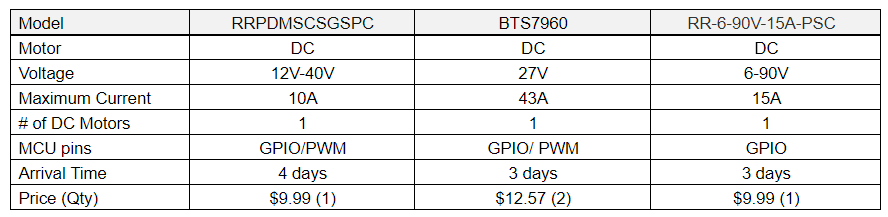
\includegraphics[width=1\textwidth]{./Images/wheel_driver_table.png}
	\caption{\label{fig:wheel_driver}Wheel Motor Driver Specifications}
\end{table}

\noindent Comparing options, we decided upon using the BTS7960 motor driver. The BTS7960 is able to supply more than enough current to the DC motors driving the wheels. This option is also the most cost-effective as the price includes two motor drivers to be able to drive both motors \cite{RioRand} \cite{Gikfun} \cite{Hobbywing}.\\ 